\documentclass[UTF8]{ctexart}
\usepackage{graphicx}
\usepackage{subfigure}
\usepackage{float}
\usepackage{geometry}
\usepackage{enumerate}
\usepackage{amsmath}
\usepackage{pgf, tikz}

\geometry{left=2.0cm, right=2.0cm, top=2.5cm, bottom=2.5cm}
\title{第二次技术文档}
\author{刘畅 15061183}

\begin{document}
	\maketitle
	% \tableofcontents
	\section{程序说明}
	\noindent
	\textbf{使用语言:} JAVA \newline
	\textbf{编程环境:} Windows 8.1 + Eclipse Neon.3 Release (4.6.3) \newline
	\textbf{相关库:}\newline
	\indent java.awt\newline
	\indent java.io\newline
	\indent java.util\newline
	\indent javax.imageio\newline
	\textbf{主要方法:} \newline
	\begin{tabular}{p{10cm}p{7cm}}
	\hline
	\textbf{方法名}& \textbf{作用} \\
	\hline
	double[][] DCTProcessor::CosineTransformation(String outputLabel) {..}&  离散余弦变换DCT\\
	\hline
	FourierComplex[][] FFTProcessor::fourierTransformation(String outputlabel) {..}&  快速傅里叶变换FFT\\
	\hline
	BufferedImage FFTProcessor::fourierInverse(String outputLabel, FourierComplex[][] sigs) {..}&  快速傅里叶逆变换IFFT\\
	\hline
	FourierComplex[][] FrequencyFilter::filter(FourierComplex[][] sigs, int radius, int mode) {..}& 高\textbackslash低频滤波,sigs为原信号,redius为滤波范围,mode值取0或1表示滤波类型 \\
	\hline
	\end{tabular}

	\section{任务一:快速傅里叶变换FFT}
		\subsection{一阶FFT}
		根据DFT,设原离散信号为$x$,转变后的信号为$X$,信号的长度为$N$,则有
		\[
			X(k) = \sum_{n=0}^{N-1}x(n)e^{-j}\frac{2\pi k}{N}n,\ k=0,1,\ldots,N-1
		\]
		假定$N \ge 2$,令$W_N^l=e^{-j\frac{2\pi l}{N}}$,则上公式可以表示成
		\[
			X(k)=\sum_{n=0}^{N-1}x(n)W_N^nk
		\]
		将上公式进行奇偶拆分,用$2r$表示偶数,$2r+1$表示奇数,$r=0,1,\ldots,N/2-1$,则有
		\[
			X(k) = \sum_{r=0}^{N/2-1}x(2r)W_{N/2}^{rk}+W_N^k\sum_{r=0}^{N/2-1}x(2r+1)W_{N/2}^{rk}
		\]
		令
		$
			G(k)=\sum_{r=0}^{N/2-1}x(2r)W_{N/2}^{rk}
		,\  
			H(k)=\sum_{r=0}^{N/2-1}x(2r+1)W_{N/2}^{rk}
		$,
		则
		\[
			X(k)=G(k)+W_N^kH(k)
		\]
		由于$G(k)$与$H(k)$周期皆为$N/2$,因此有
		\[
			X(k)=\left\{
			\begin{array}{lcl}
			G(k) + W_N^kH(k) & & ,{0 \leq k < N/2} \\
			G(k-N/2)-W_N^{k-N/2}H(k-N/2) & & ,{N/2 \leq k < N} \\
			\end{array}
			\right.
		\]
		\indent以$G(k)$为例,假定$N \ge 4$,同样可以进行类似的拆分,转化为由$GG(k)$和$GH(k)$组成的表达式
		\[
			\begin{aligned}
			G(k) &= \sum_{r=0}^{N/4-1}x(4r)W_{N/4}^{rk} + \sum_{r=0}^{N/4-1}x(4r+2)W_{N/4}^{rk} \\
			&= GG(k) + W_{N/2}^{rk}GH(k) \\
			&= \left\{
			\begin{array}{lcl}
			GG(k) + W_{N/2}^kGH(k) & & ,{0 \leq k < N/4} \\
			GG(k-N/4)-W_{N/2}^{k-N/4}GH(k-N/4) & & ,{N/4 \leq k < N/2} \\
			\end{array}
			\right.
			\end{aligned}
		\]
		以此类推,通过不断的奇偶拆分,最终可以形成由$x$至$X$的蝶形结构,如图\ref{fft-btf}所示,这里假定$N \ge 8$:
		\begin{figure}[]
			\centering
			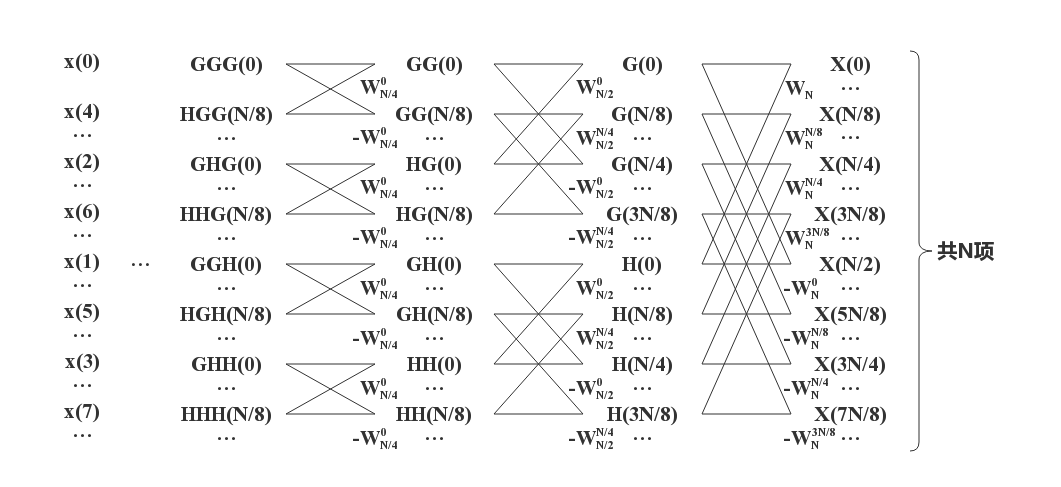
\includegraphics[width=1\textwidth]{fft.png}
			\caption{FFT蝶形结构}
			\label{fft-btf}
		\end{figure}

	\subsection{图像FFT}
		由于需要处理的图像是一种二维数字信号,因此上述FFT算法需要扩展到二维。这里采用的方法是将图像看成一个二维矩阵,首先对各行进行FFT处理,之后再对各列进行FFT处理,这样就将一维FFT扩展到了二维。
		而且需要注意的是,FFT算法能够进行的前提是信号长度$N$为2的正整数幂,因此图像需要进行周期延拓,最终处理后矩阵长、宽皆变为2的正整数幂。

	\subsection{生成频域图像}
		处理后的矩阵为复数矩阵,根据以下公式求出幅度谱$|F(u,v)|$和相位谱$\phi(u,v)$:
		\[
			|F(u,v)| = \sqrt{R^2(u,v) + I^2(u,v)}
		\]
		\[
			\phi(u,v) = \textrm{tan}^{-1}\frac{I(u,v)}{R(u,v)}
		\]
		\indent计算后矩阵上各个元素的幅度差异较大,存在少量高幅信号和大量低幅信号,若将幅度线性映射至灰度,生成的幅度谱信息量较少。为解决该问题,同时保证滤波后频谱图像效果的一致性,这里对幅度设定了阈值$T$,对于大于$T$的幅度,其映射后的灰度为255;对于小于$T$的,部分在$[0,255]$范围内做线性映射,这里用$f(u,v)$表示灰度,假设最低幅度为$F_{\textrm{min}}$,最高幅度为$F_{\textrm{max}}$,则有
		\[
			f(u,v) = \left\{
				\begin{array}{lcl}
				\frac{255(|F(u,v)|-F_{\textrm{min}})}{\textrm{min}\{F_{\textrm{max}},T\}-F_{\textrm{min}} } & &, {|F(u,v)| \leq T} \\
				255 & &, {|F(u,v)| > t}
				\end{array}
			\right.
		\]
		在不对相位谱进行平移的情况下,亮点主要集中于四角,为了便于观察,需要将亮点移动至图像中心。

		\begin{figure}[htbp]
		\centering
		\subfigure[原图]{
			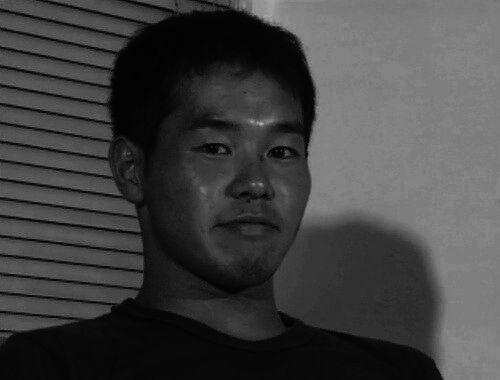
\includegraphics[width=0.3\textwidth]{grey_grey.png}} \\
		\subfigure[幅度谱]{
			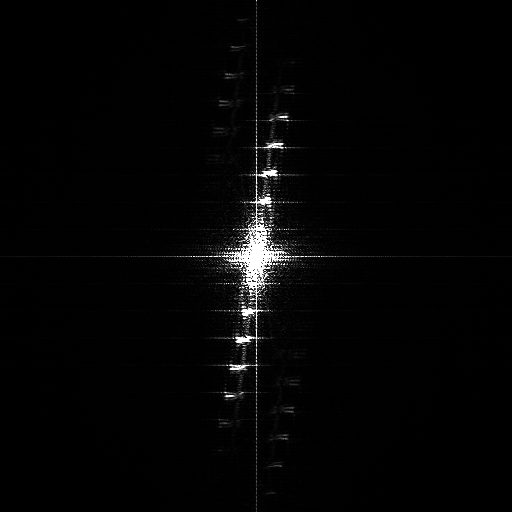
\includegraphics[width=0.3\textwidth]{FFT_Range_trans.png}}
		\subfigure[相位谱]{
			
\includegraphics[width=0.3\textwidth]{FFT_Phase_trans.png}}
		\caption{某24岁学生FFT变换后效果}
		\end{figure}

	\subsection{逆变换IFFT}
		离散傅里叶反变换IDFT公式为:
		\[
			x(n) = \frac{1}{N}\sum_{k=0}^{N-1}X(k)e^{j\frac{2\pi k}{N}n}
		\]
		与DFT不同的是IDFT需要额外乘以常量$\frac{e^{-1}}{N}$,因此对于IFFT可以复用上述蝶形求解方式,无需额外实现。
		\indent由于逆变换前的矩阵为延拓后的结果,因此需要根据图像实际大小,对逆变换后的结果进行截取。同时,理论上逆变换后矩阵的元素应为实数,但由于在浮点数计算的过程中存在精度丢失的情况,可能会导致元素虚部不为0,或者实部大小不在$[0,255]$范围内,此时应当将实部线性压缩,保证灰度的合法性。

	\subsection{滤波}
		对于平移后的频谱,设图像中央为原点,截止频率$D_0$,则理想低通滤波器转移函数为:
		\[
			H(u,v) = \left\{
			\begin{array}{lcl}
			1 & &, {\sqrt{u^2+v^2} < D_0} \\
			0 & &, {\sqrt{u^2+v^2} \ge D_0}
			\end{array}
			\right.
		\]
		理想高通滤波器转移函数为:
		\[
			H(u,v) = \left\{
			\begin{array}{lcl}
			0 & &, {\sqrt{u^2+v^2} < D_0} \\
			1 & &, {\sqrt{u^2+v^2} \ge D_0}
			\end{array}
			\right.
		\]

		\begin{figure}[]
		\centering
		\subfigure[原图]{
			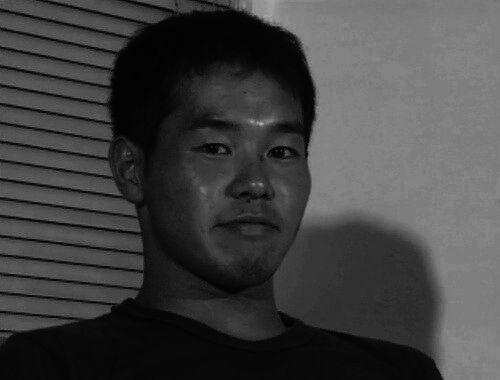
\includegraphics[width=0.3\textwidth]{grey_grey.png}} \\
		\subfigure[$D_0=50$图像]{
			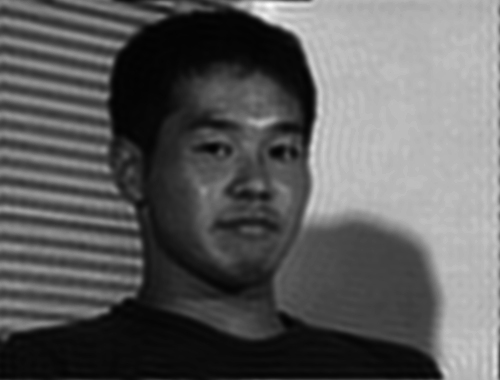
\includegraphics[width=0.3\textwidth]{FFT_Inverse_inverse_50_1.png}}
		\subfigure[$D_0=20$图像]{
			
\includegraphics[width=0.3\textwidth]{FFT_Inverse_inverse_20_1.png}}
		\subfigure[$D_0=10$图像]{
			
\includegraphics[width=0.3\textwidth]{FFT_Inverse_inverse_10_1.png}}
		\subfigure[$D_0=50$幅度谱]{
			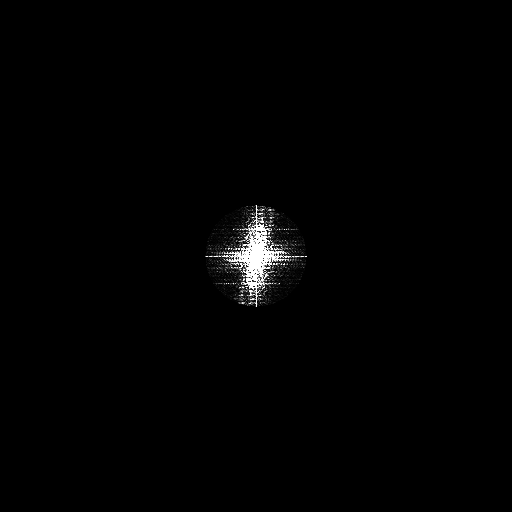
\includegraphics[width=0.3\textwidth]{FFT_Range_inverse_50_1.png}}
		\subfigure[$D_0=20$幅度谱]{
			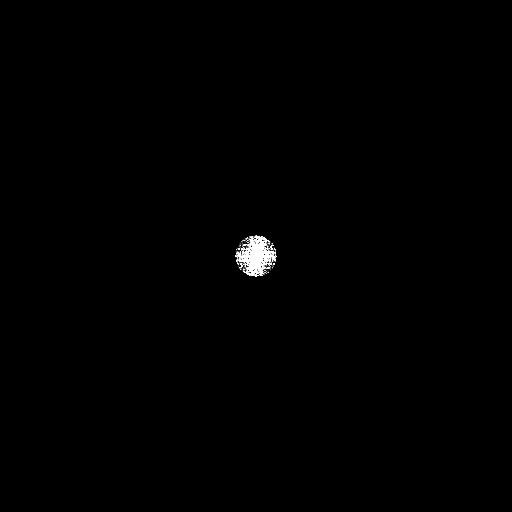
\includegraphics[width=0.3\textwidth]{FFT_Range_inverse_20_1.png}}
		\subfigure[$D_0=10$幅度谱]{
			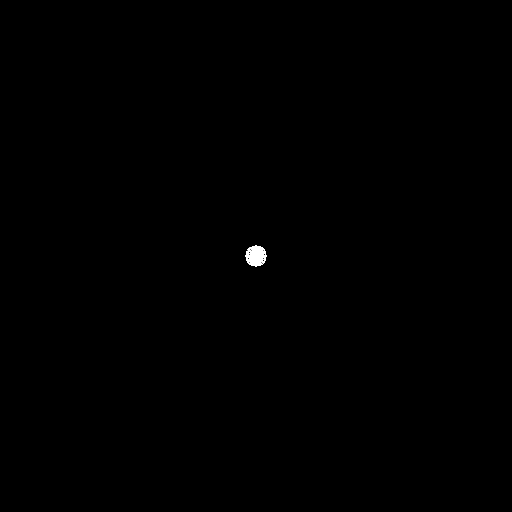
\includegraphics[width=0.3\textwidth]{FFT_Range_inverse_10_1.png}}
		\caption{低通滤波后效果}
		\end{figure}

		\begin{figure}[]
		\centering
		\subfigure[原图]{
			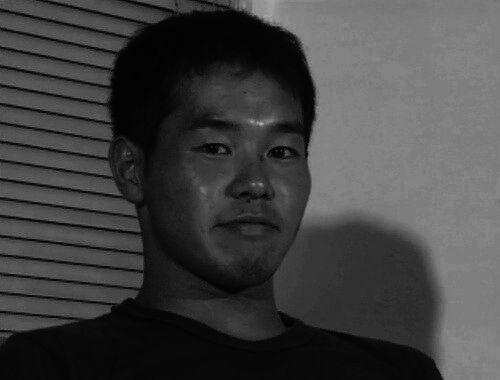
\includegraphics[width=0.3\textwidth]{grey_grey.png}} \\
		\subfigure[$D_0=20$图像]{
			
\includegraphics[width=0.3\textwidth]{FFT_Inverse_inverse_20_0.png}}
		\subfigure[$D_0=10$图像]{
			
\includegraphics[width=0.3\textwidth]{FFT_Inverse_inverse_10_0.png}}
		\subfigure[$D_0=5$图像]{
			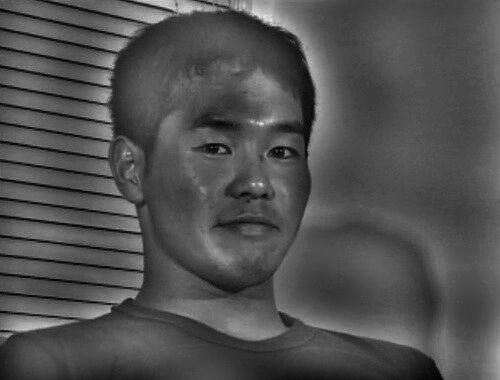
\includegraphics[width=0.3\textwidth]{FFT_Inverse_inverse_5_0.png}}
		\subfigure[$D_0=20$幅度谱]{
			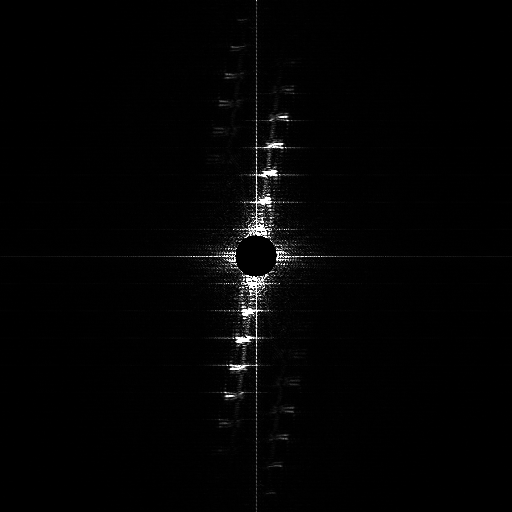
\includegraphics[width=0.3\textwidth]{FFT_Range_inverse_20_0.png}}
		\subfigure[$D_0=10$幅度谱]{
			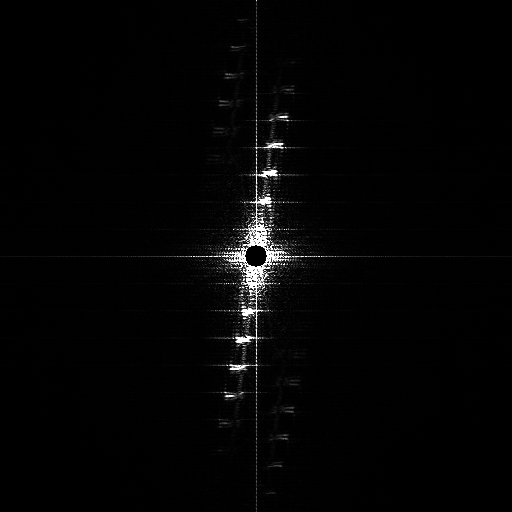
\includegraphics[width=0.3\textwidth]{FFT_Range_inverse_10_0.png}}
		\subfigure[$D_0=5$幅度谱]{
			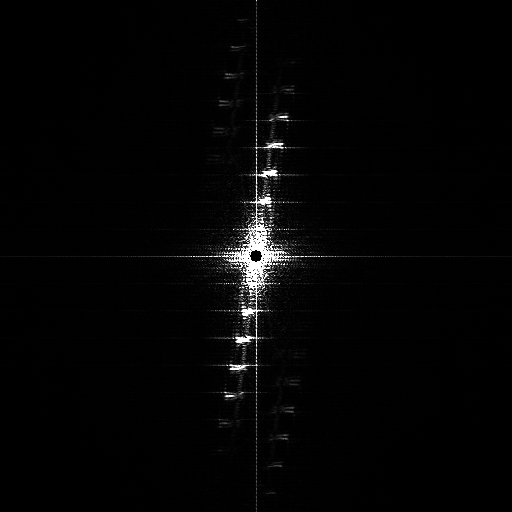
\includegraphics[width=0.3\textwidth]{FFT_Range_inverse_5_0.png}}
		\caption{高通滤波后效果}
		\end{figure}

	\section{任务二:离散余弦变换DCT}
		\subsection{一维DCT}
			设$k=1,2,\ldots,N-1$一维DCT定义如下:
			\[
				X(k) = C(k)\sqrt{\frac{2}{N}}\sum_{n=0}^{N-1}\textrm{cos}\frac{(2n+1)k\pi}{2N},\ C(k)=\left\{
				\begin{array}{lcl}
				\frac{1}{\sqrt{2}} &&, {u = 0}\\
				1 &&, {\textrm{other}}
				\end{array}
				\right.
			\]
		\subsection{图像DCT}
			同FFT一样,二维DCT同样可以通过横纵两次一维DCT来完成,和FFT不同的是无需对信号进行延拓,且结果为实数,因此最终得到的是一个和原信号大小相同的实数矩阵。
			\indent最终的结果主要信息集中在画面的左上角,为了显示更多信息,这里同样设置了一个阈值$T$,采用和FFT同样的方法进行从信号到灰度的线性映射。
			\begin{figure}[]
			\centering
			\subfigure[原图]{
				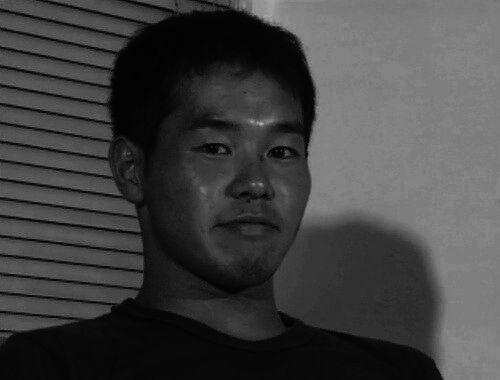
\includegraphics[width=0.3\textwidth]{grey_grey.png}} 
			\subfigure[DCT频域图]{
				
\includegraphics[width=0.3\textwidth]{DCT_trans.png}}
			\caption{DCT变换后效果}
			\end{figure}

\end{document}